\section{Count of persons data}

\subsection{Properties of the data}
\label{sec:PassengerDensityData}

In order to model the passenger density an understanding of the available data is necessary. In this section the data, visible pattern and other features are discussed.

Figure~\ref{fig:rawData_week} illustrates exemplary the available values of a camera and week. The PdG service times are visible due to the low passenger density level between 01:00 and 05:00 on weekdays.
\marginpar{
\begin{figure}%[htbp]
  \begin{center}
  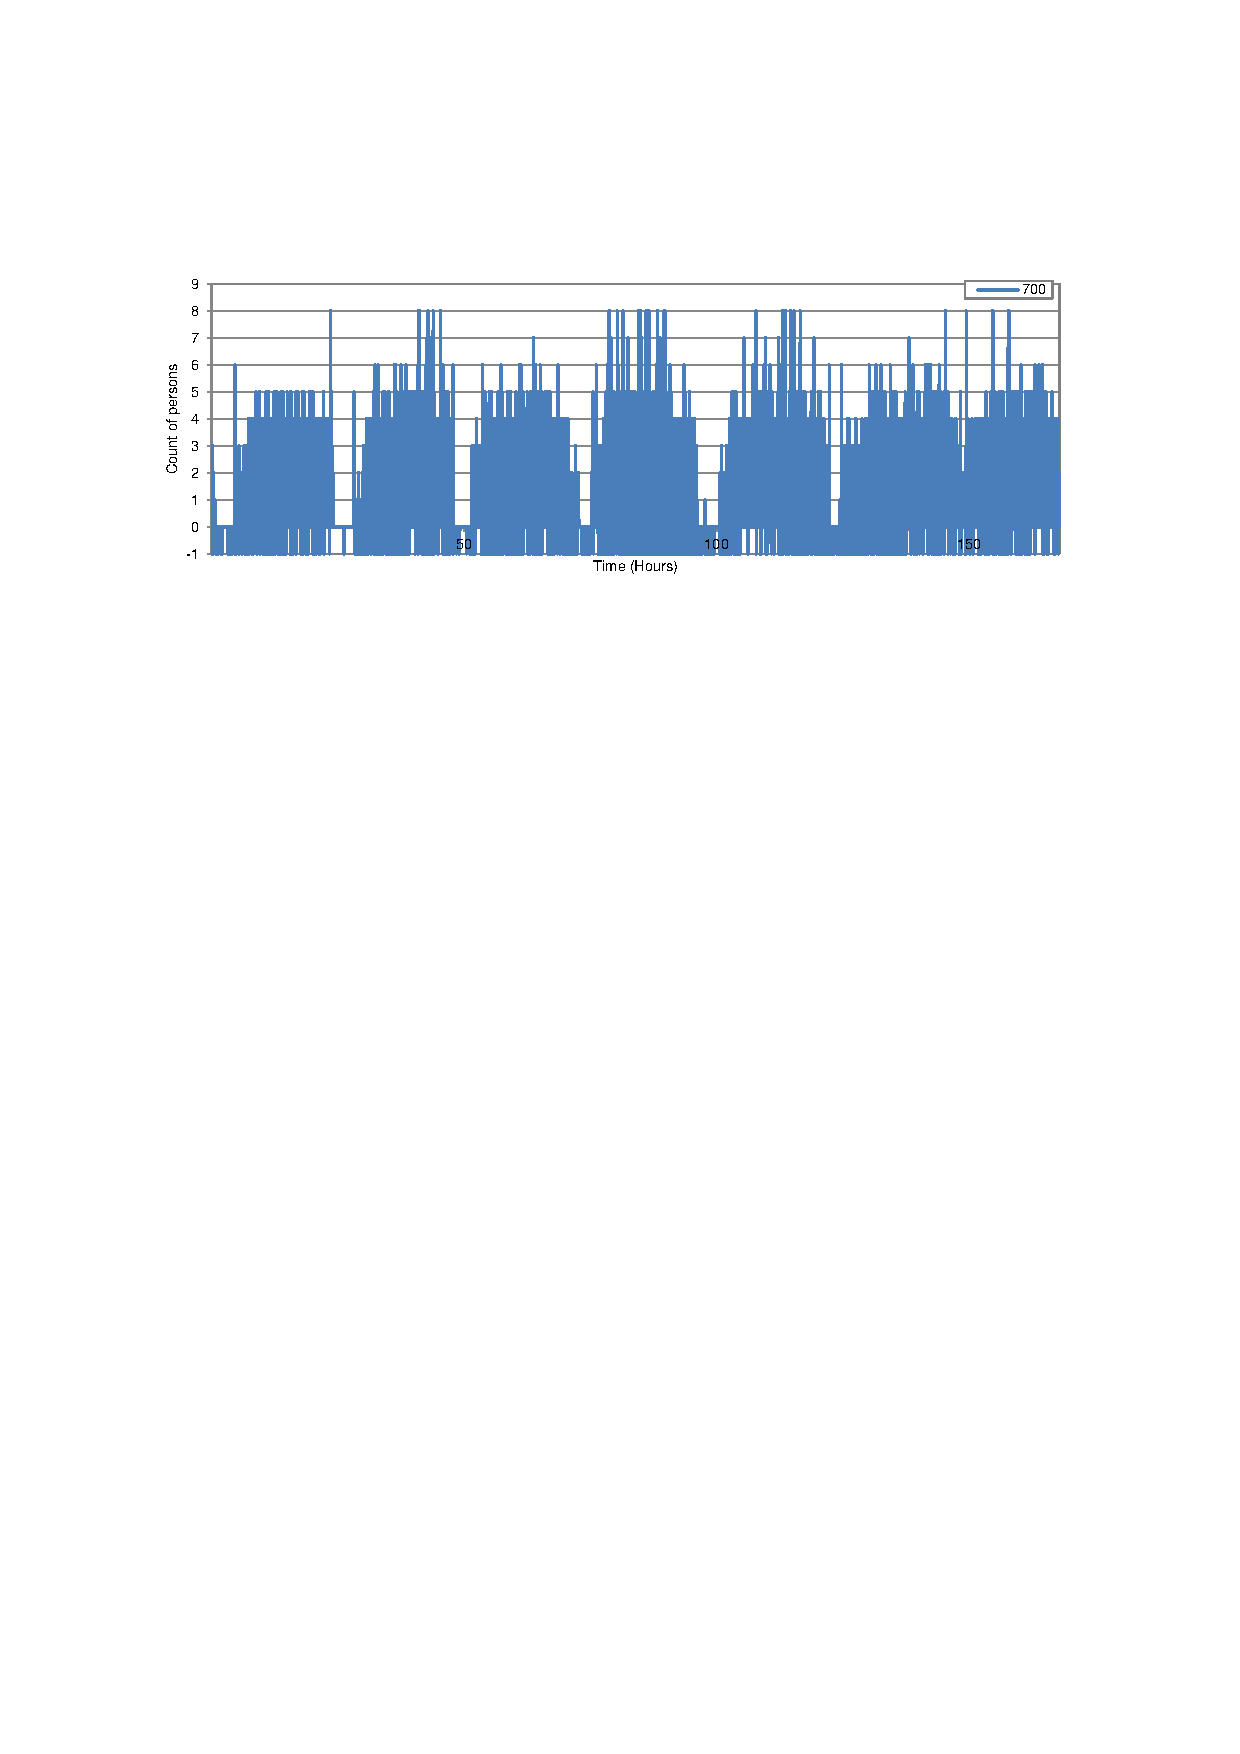
\includegraphics[height=\marginparwidth, angle=90]{Figures/rawData_week.pdf}
  \caption{Passenger density distribution of one camera during one week.}
  \label{fig:rawData_week}
  \end{center}
\end{figure}
}

\begin{figure*}
\centering
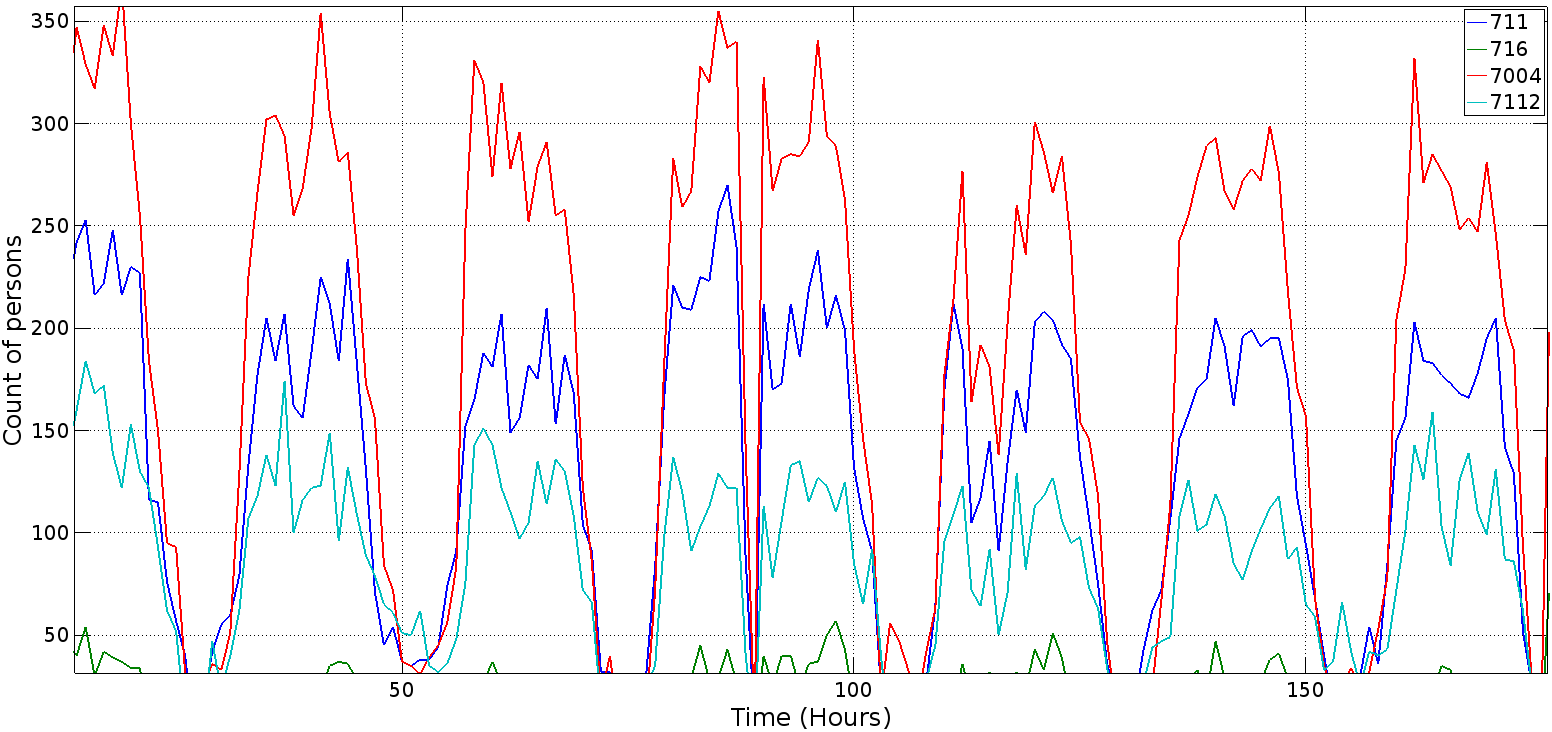
\includegraphics[width=\textwidth]{Figures/Figure_PersonCount_Hours.png}
 \caption{todo}
\end{figure*}

\subsection{Prediction by Artificial Neural Fuzzy Inference System}

\begin{figure*}
\centering
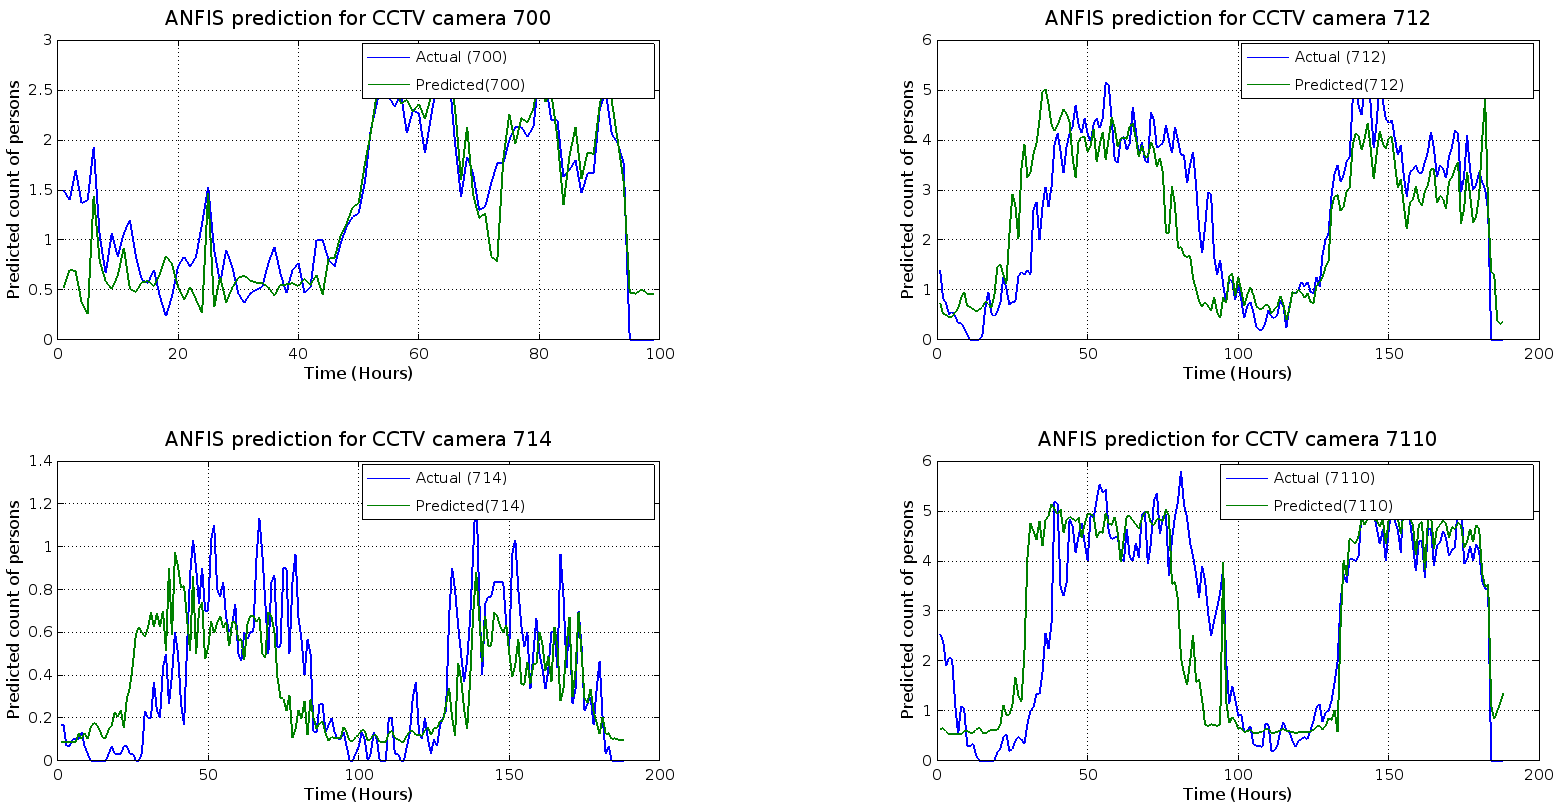
\includegraphics[width=\textwidth]{Figures/Figure_Prediction.png}
 \caption{todo}
\end{figure*}

\begin{figure*}
\centering
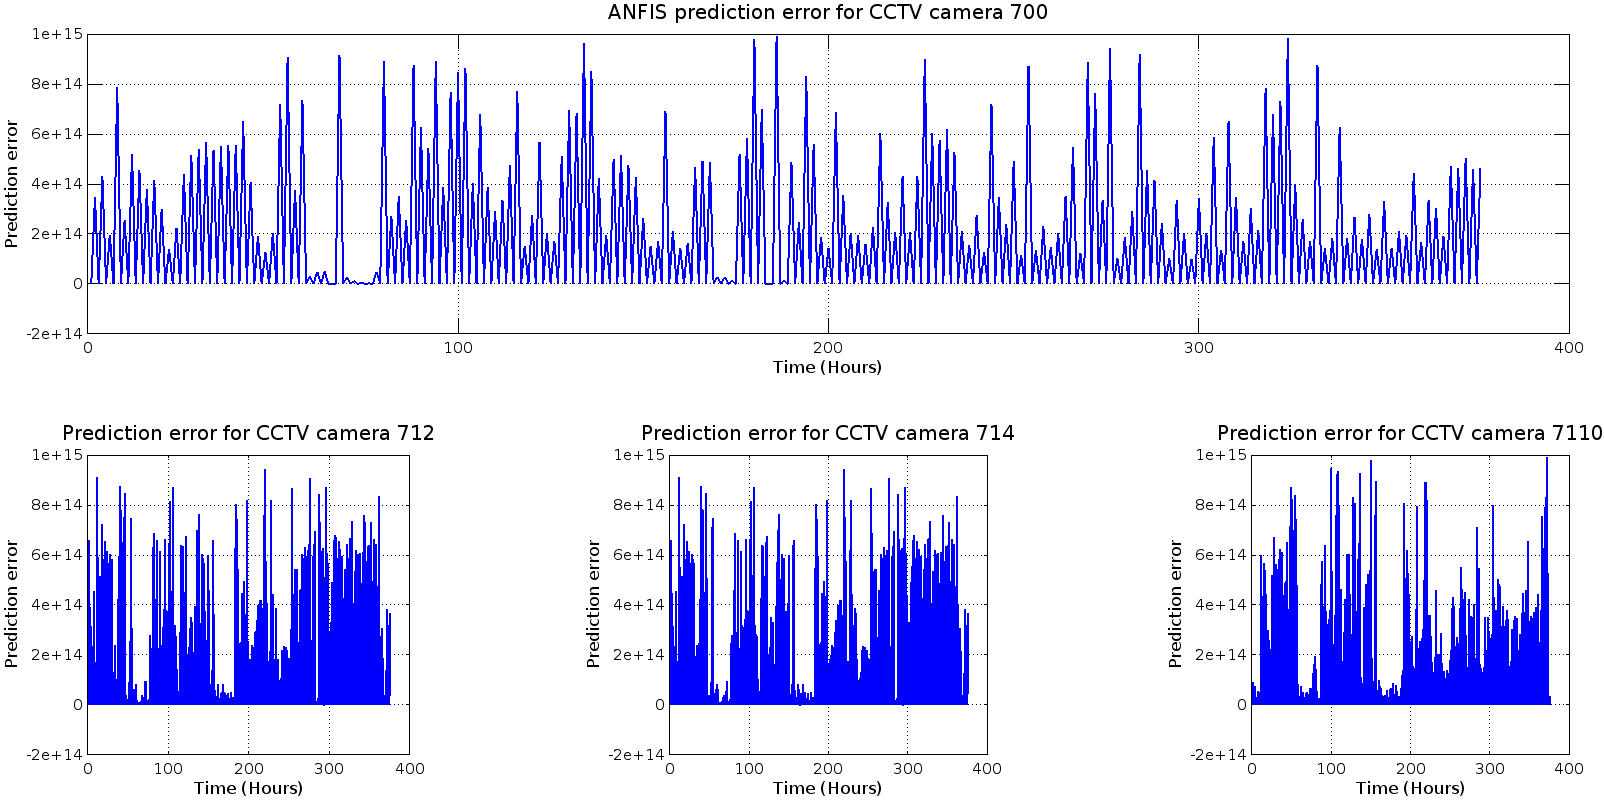
\includegraphics[width=\textwidth]{Figures/Figure_PredictionError.png}
 \caption{todo}
\end{figure*}

